\documentclass[12pt,a4paper]{article} 

\usepackage{float,times,graphicx,mathtools}
\usepackage{amsmath}
\usepackage{amsfonts}
\usepackage{amssymb}
\usepackage{latexsym}
\usepackage{epsfig}
\usepackage{graphicx}
\usepackage{caption}
\usepackage{subcaption}
\usepackage{color}
\usepackage{pdfpages}
\usepackage{natbib}
\usepackage[space]{grffile}
\usepackage{wrapfig}
\usepackage{subcaption}
\usepackage{url}
\usepackage{bbm}
\usepackage{tikzsymbols}

\DeclareMathOperator{\logit}{logit}
\DeclareMathOperator{\tr}{tr}
\bibpunct[, ]{(}{)}{;}{a}{,}{,}
\graphicspath{{../Burkina Faso/12/}}  
\addtolength{\oddsidemargin}{-1in}
	\addtolength{\evensidemargin}{-1in}
	\addtolength{\textwidth}{1.75in}
	\addtolength{\topmargin}{-1.3in}
	\addtolength{\textheight}{2in}
\date{\vspace{-5ex}}

\begin{document}
Prior for spline coefficients $\boldsymbol{\beta} \sim \sqrt{\tau^{-1}} AR2(2\rho, -\rho), \quad \rho \in (0, 1)$, where $AR2$ is standardised with marginal variances $= 1.$

\paragraph{PC priors for $\rho$} \\~\\

Assuming $\boldsymbol{\beta}$ follows an AR2 process with $\boldsymbol{\rho} = (2\rho, -\rho)$, with $\rho \in (0, 1)$ and let $\boldsymbol{\Sigma}$ be the corresponding correlation matrix, i.e. marginal variances of $\boldsymbol{\beta} = 1$. Then the KLD for the construction of the PC prior for $\rho$, assuming base model is $\rho = 0$ (i.e. an i.i.d Normal), is:

\begin{align*}
KLD(f_1 \Vert f_0) = \frac{1}{2} \Bigg( \text{tr}(\boldsymbol{\Sigma_0^{-1} \Sigma_1}) - n - \log \Big( \frac{\vert  \boldsymbol{\Sigma_1} \vert}{\vert \boldsymbol{\Sigma_0} \vert} \Big) \Bigg)
\end{align*}
Since the base model is $\rho = 0$, $\boldsymbol{\Sigma_0} = \boldsymbol{I}$ and hence $\text{tr}(\boldsymbol{\Sigma_0^{-1}\Sigma_1}) = \text{tr}(\boldsymbol{\Sigma_1}) = n$, since $\boldsymbol{\Sigma_1}$ is a correlation matrix.

\begin{align*}
\implies KLD(f_1 \Vert f_0) &= -\frac{1}{2} \log(\vert \boldsymbol{\Sigma_1} \vert) \\
&= -\frac{1}{2} \log \big[ \, (1-\psi_1^2)^{n-1} (1-\psi_2^2)^{n-2} \, \big] \\
&= -\frac{1}{2} \log \big[ \, (1- \big(\frac{2\rho}{1+\rho}\big)^2 )^{n-1} (1-\rho^2)^{n-2}\, \big] \\
&= -\frac{1}{2} \log \big[\, (1+3\rho)^{n-1} (1-\rho)^{2n-3} (1+\rho)^{-n}  \, \big]
\end{align*}


The PC prior is defined as an exponential prior on $d(\rho) = \sqrt{2 KLD(f_1 \Vert f_0)}$ with rate $\lambda$.

Consider 
\begin{align*}
d(\rho) &= \sqrt{2 KLD(f_1 \Vert f_0)} \\
&= \sqrt{- \log \big[ \, (1- \big(\frac{2\rho}{1+\rho}\big)^2 )^{n-1} (1-\rho^2)^{n-2}\, \big]} \tag{1}\\
&= \sqrt{(1-n) \log(1+3\rho) + (3-2n) \log(1-\rho) + n \log(1+\rho)}\\
&= \sqrt{f(\rho)},
\end{align*}
then 
\begin{align*}
\frac{\partial d(\rho)}{\partial\rho} &= \frac{1}{2\sqrt{f(\rho)}} \Big[\, \frac{3-3n}{1+3\rho} + \frac{2n-3}{1-\rho} + \frac{n}{1+\rho} \,\Big] \\
&= \frac{1}{2\sqrt{f(\rho)}} \Big[\, \frac{(3-3n)(1-\rho)(1+\rho) + (2n-3)(1+3\rho)(1+\rho) + n(1+3\rho)(1-\rho)}{(1+3\rho)(1-\rho)(1+\rho)}   \,\Big] \\
&= \frac{1}{2\sqrt{f(\rho)}} \Big[\, \frac{\rho^2(6n-12) + \rho(10n - 12)}{(1+3\rho)(1-\rho)(1+\rho)}\,\Big] > 0 \qquad \qquad \forall \rho \in (0, 1),
\end{align*}
i.e. $d(\rho)$ is a monotonically increasing positive function in $\rho$, which is intuitive as $\rho \to 1$ means higher deviation from the base model $\rho = 0$ and hence higher KLD. 

Thus, PC prior for $\rho$ is
\begin{align*}
\pi(\rho) &= \pi_{d}(d(\rho)) \Big \vert \frac{\partial d(\rho)}{\partial\rho} \Big \vert \\
&= \lambda_{\rho} e^{-\lambda_{\rho} d(\rho)} \, \frac{\partial d(\rho)}{\partial \rho}
\end{align*}

To determine the decay rate $\lambda_{\rho}$, the authors suggested inferring from a interpretable probability statement $P(Q(\rho) > U) = \alpha$ for some $\alpha$ as the tail probability. Here I plan to directly work on the $\rho$ scale, e.g. specifying $P(\rho > 0.99) = 0.01$ as a loose PC prior. Since $d(\rho)$ is a monotonically increasing one-to-one mapping, the upper bound specified on $\rho$ can be translated into an upper for $d(\rho)$ as $P(d(\rho) > d(U)) = 0.01$. Knowing the tail probability of an exponential R.V $P(X > x) = 1 - \text{c.d.f}(x) = e^{-\lambda x}$, $\lambda_\rho$ can be derived from $e^{-\lambda_{\rho} d(U)} = 0.01 \implies \lambda_\rho = -\log(0.01) / d(U)$.

\paragraph{PC prior for $\tau$} \\~\\

If information is available on the variability on the spline coefficients, the PC prior for $\tau$ can be inferred directly by a similar procedure of setting an upper bound for $\tau$, however the scale of $\tau$ often depends on several factors, e.g. the spacing of the knots, the scale of the problem, etc. To see this, consider $y = \boldsymbol{B\beta}$ where $\boldsymbol{B}$ is the design matrix, then $\text{VAR}(y) = \tau^{-1}\boldsymbol{B \Sigma_1(\rho) B'}$. Therefore the scale of $\tau$ depends on $\rho$. The diagonal of the matrix $\boldsymbol{B \Sigma_1(\rho) B'}$ is relatively uniform, due to the stationarity of the AR2 process assumed and the equal knot spacing and even data. To simplify the construction, we approximate the marginal variance of each $y_i = \text{VAR}(y_1) = \tau^{-1} \boldsymbol{B_{1\cdot}\phantom{'} \, \Sigma_1{(\rho)} \, B'_{1\cdot}}$, where $\boldsymbol{B_{1\cdot}\phantom{'}}$ is the first row of the design matrix. It is usually easier to give probability statements on the standard deviation of $\boldsymbol{y}$ instead of $\boldsymbol{\beta}$. Hence, the PC prior for $\tau$ is the type-2 Gumbel prior with decay rate $\lambda_{\tau} = -\log(0.01) \sqrt{\text{VAR}(y_1)}/ U_{y}$, where $U_y$ is an upper bound of the standard deviation of $y$.

Therefore
\begin{align*}
f(\tau, \rho) &= f(\tau | \rho) f(\rho) \\
&= \text{type-2 Gumbel}(\tau, \lambda_{\tau}|\rho) \cdot \pi(\rho) \\
&= \text{type-2 Gumbel}(\tau, \lambda_{\tau}|\rho) \cdot  \lambda_{\rho} e^{-\lambda_{\rho} d(\rho)} \, \frac{\partial d(\rho)}{\partial \rho}
\end{align*}

The dependence of $\lambda_{\tau}$ on $\rho$ is through $\text{VAR}(y_1)$.

\paragraph{PC prior for a different variance for the HIV period} \\~\\
It may be more logical to have a different variance, especially for the hump component, during the HIV epidemics. For example, if we have $\boldsymbol{\eta} \sim AR2$, then we can assume $\boldsymbol{\beta} = \boldsymbol{\sqrt{W}\eta} \sim \boldsymbol{\sqrt{W}} AR2$, where $\boldsymbol{W}$ is a diagonal matrix with elements equal to the marginal variances of each $\beta$'s. For simplicity, I set $\boldsymbol{W} = \text{diag}(w_1, w_1, w_1, \dots, w_2, w_2, w_2)$, i.e. constant variance before the epidemics and another constant variance after. Obviously, this would destroy the stationarity of the AR2, but it is sensible and hence desirable, as we would not expect the stationarity to hold during the epidemics. Under this formulation, the $\beta$'s in the pre-HIV era still enjoys stationarity.

It is slightly more difficult to set up the PC prior for $w_2$. To proceed, I re-parameterise the model such that 

\begin{align*}
\boldsymbol{\beta} = \sqrt{w_1} \begin{pmatrix}
																	1 & 0 & 0 & 0 & \dots \\
																	0 & 1 & 0 & 0 & \dots \\
																	\vdots & \ddots & & & \\
																	& & \sqrt{\gamma} & 0 & 0 \\
																	& & 0 & \sqrt{\gamma} & 0 \\
																	& & 0 & 0 & \sqrt{\gamma}
																	\end{pmatrix} \boldsymbol{\eta},
\end{align*}
where $\boldsymbol{\eta}$ follows an AR2($2\rho, -\rho$) process with marginal variances $= 1$. Under this parameterisation, we could write the prior $\pi(w_1, \gamma, \rho) = \pi(w_1 | \gamma, \rho) \pi(\gamma | \rho) \pi(\rho)$, where $\pi(\rho)$ is the same as above as it does not depend on the variance parameters (since it relates to a correlation matrix), and $\pi(w_1^{-1} | \gamma, \rho)$ has a gumbel density as above, because Simpson et al. showed the PC prior of it is independent on the covariance matrix, after conditioning on $\gamma$ and $\rho$.

To calculate the PC prior for $\gamma$, again we consider the $KLD(f_1 \Vert f_0)$, where the base model $f_0$ is now at $\gamma = 1$, i.e. same variance for the whole period. It can also be seen that under this formulation we can set the prior for $\gamma$ independent of $w_1$, as the $w_1$ in the base model and the alternative model cancel out.
\begin{align*}
KLD(f_1 \Vert f_0) &= \frac{1}{2} \Bigg( \text{tr}(\boldsymbol{\Sigma_0^{-1} \Sigma_1}) - n - \log \Big( \frac{\vert  \boldsymbol{\Sigma_1} \vert}{\vert \boldsymbol{\Sigma_0} \vert} \Big) \Bigg) \\
 &= \frac{1}{2} \Bigg( \text{tr}(\boldsymbol{\Sigma_0^{-1} \sqrt{W} \Sigma_0 \sqrt{W}})- n - \log \Big( \frac{\vert  \boldsymbol{\sqrt{W}\Sigma_0 \sqrt{W}} \vert}{\vert \boldsymbol{\Sigma_0} \vert} \Big) \Bigg)  \\
&= \frac{1}{2} \Bigg( \text{tr}(\boldsymbol{\Sigma_0^{-1} \sqrt{W} \Sigma_0 \sqrt{W}}) - n - (n_{\gamma})\log(\gamma) \Bigg),
\end{align*}
where $n_{\gamma}$ indicates the number of $\beta$'s with the different variance.

The first term requires more attention. Using the block matrix inversion formula, write:
\begin{align*}
&\text{tr}\big(\boldsymbol{\boldsymbol{\Sigma_0^{-1} \sqrt{W} \Sigma_0} \sqrt{W}}\big) = \text{tr}\bigg(\begin{pmatrix} \boldsymbol{A} & \boldsymbol{B} \\
\boldsymbol{C} & \boldsymbol{D} \end{pmatrix}^{-1} \begin{pmatrix} \boldsymbol{I} & \boldsymbol{0} \\
\boldsymbol{0} & \sqrt{\gamma}\boldsymbol{I} \end{pmatrix} \begin{pmatrix} \boldsymbol{A} & \boldsymbol{B} \\
\boldsymbol{C} & \boldsymbol{D} \end{pmatrix} \begin{pmatrix} \boldsymbol{I} & \boldsymbol{0} \\
\boldsymbol{0} & \sqrt{\gamma}\boldsymbol{I} \end{pmatrix} \bigg)\\
= \text{tr}\Bigg(&\begin{pmatrix} \boldsymbol{A^{-1} + A^{-1}B(D-CA^{-1}B)^{-1}CA^{-1}} & \boldsymbol{-A^{-1}B(D-CA^{-1}B)^{-1}} \\
\boldsymbol{-(D-CA^{-1}B)^{-1}CA^{-1}} & \boldsymbol{(D-CA^{-1}B)^{-1}} \end{pmatrix} \begin{pmatrix} \boldsymbol{A} & \sqrt{\gamma}\boldsymbol{ B} \\
\sqrt{\gamma}\boldsymbol{ C} & \gamma\boldsymbol{D} \end{pmatrix}\Bigg) \\
= \text{tr} \big(& \boldsymbol{I + A^{-1}B(D-CA^{-1}B)C} - \sqrt{\gamma}\boldsymbol{A^{-1}B(D-CA^{-1}B)C} \big) + \\
& \qquad \qquad \qquad \qquad \qquad \text{tr} \big( -\sqrt{\gamma}\boldsymbol{(D-CA^{-1}B)CA^{-1}B} + \gamma\boldsymbol{(D-CA^{-1}B)D} \big) \\
\text{using}& \text{ the cyclic property,} \\
= \text{tr} \big(& \boldsymbol{I} \big) + (1-2\sqrt{\gamma}) \, \text{tr} \big( \boldsymbol{(D-CA^{-1}B)CA^{-1}B} \big) + \gamma \, \text{tr} \big(\boldsymbol{(D-CA^{-1}B)^{-1}D} \big) \\
= \text{tr} \big(& \boldsymbol{I} \big) + (1-2\sqrt{\gamma}) \, \text{tr} \big( \boldsymbol{(D-CA^{-1}B)CA^{-1}B} \big) + \gamma \, \text{tr} \big(\boldsymbol{(D-CA^{-1}B)^{-1}D} \big) + \\
&\qquad \qquad \qquad \qquad \gamma \, \text{tr} \big(\boldsymbol{(D-CA^{-1}B)^{-1}CA^{-1}B} \big) - \gamma \, \text{tr} \big(\boldsymbol{(D-CA^{-1}B)^{-1}CA^{-1}B} \big) \\
= \text{tr} \big(& \boldsymbol{I} \big) +  \gamma \, \text{tr} \big( \boldsymbol{I}_{n_{\gamma}} \big) + (1-2\sqrt{\gamma} + \gamma) \, \text{tr} \big( \boldsymbol{(D-CA^{-1}B)CA^{-1}B} \big)\\
= \text{tr} \big(& \boldsymbol{W} \big) +  (1 - \sqrt{\gamma})^2 \, \text{tr} \big( \boldsymbol{(D-CA^{-1}B)CA^{-1}B} \big)\\
= \text{tr} \big(& \boldsymbol{W} \big) +  (1 - \sqrt{\gamma})^2 \, \text{tr} \big( \boldsymbol{EB} \big)\\
\end{align*}
By comparing term of the block inversion formula, it is easily seen that $-\boldsymbol{E} = -\boldsymbol{(D-CA^{-1}B)CA^{-1}}$ is the bottom left block matrix of the AR2 precision matrix, and $\boldsymbol{B}$ is the upper right block matrix of the AR2 covariance matrix. Since the precision matrix of an AR2 process is a band $2 \cdot (2+1) - 1$ matrix, $\boldsymbol{E}$ is a sparse right triangular matrix with only three non-zero entries:

\begin{align*}
-\boldsymbol{E} &= \begin{pmatrix}
0 & 0 & 0 & \dots & 0 & -\phi_2 \sigma^{-2} & \phi_1 (\phi_2 - 1) \sigma^{-2} \\
0 & 0 & 0 & \dots & 0 & 0 & -\phi_2 \sigma^{-2} \\
0 & 0 & 0 & \dots 
\end{pmatrix},
\end{align*}

where $\sigma^{2}$ is the ratio of adjustment of the innovations at $t>2$ relative to the first two innovations in order to maintain stationarity. $\sigma^2 = \frac{1+\phi_2}{1-\phi_2}((1-\phi_2)^2 - \phi_1^2)$ for an AR2 process. Given $\phi_1 = 2\rho$ and $\phi_2 = -\rho$, $-\boldsymbol{E}$ reduces to

\begin{align*}
-\boldsymbol{E} &= \begin{pmatrix}
0 & 0 & 0 & \dots & 0 & \frac{\rho (1+\rho)}{(1+3\rho)(1-\rho)^{2}} & \frac{-2\rho (1+\rho)^2}{(1+3\rho)(1-\rho)^{2}}\\
0 & 0 & 0 & \dots & 0 & 0 &  \frac{\rho (1+\rho)}{(1+3\rho)(1-\rho)^{2}}  \\
0 & 0 & 0 & \dots 
\end{pmatrix}. 
\end{align*}

Therefore,
\begin{align*}
\text{tr} \big( \boldsymbol{EB} \big) = \frac{-\rho (1+\rho)}{(1+3\rho)(1-\rho)^{2}} \text{ACF}(2) + \frac{2\rho (1+\rho)^2}{(1+3\rho)(1-\rho)^{2}} \text{ACF}(1) + \frac{-\rho (1+\rho)}{(1+3\rho)(1-\rho)^{2}} \text{ACF}(2),
\end{align*}
where $\text{ACF}(\cdot)$ is the auto-correlation function. For AR2,
\begin{align*}
\text{ACF}(1) &= \frac{\phi_1}{1-\phi_2} = \frac{2\rho}{1+\rho} \\
\text{ACF}(2) &= \phi_1 \text{ACF}(1) + \phi_2 = \frac{\rho(3\rho-1)}{1+\rho} \\
\implies \text{tr}\big(\boldsymbol{EB} \big) &= \frac{2\rho (1+\rho)^2}{(1+3\rho)(1-\rho)^{2}} \text{ACF}(1) - \frac{2\rho (1+\rho)}{(1+3\rho)(1-\rho)^{2}} \text{ACF}(2)\\
&=  \frac{2\rho (1+\rho)^2}{(1+3\rho)(1-\rho)^{2}} \Big(\frac{2\rho}{1+\rho}\Big) - \frac{2\rho (1+\rho)}{(1+3\rho)(1-\rho)^{2}}  \Big(\frac{\rho(3\rho-1)}{1+\rho}\Big) \\
&= \frac{2\rho^2 (1+\rho)}{(1+3\rho)(1-\rho)^{2}} \Big ( (1+\rho) \frac{2}{1+\rho} - \frac{3\rho-1}{1+\rho} \Big) \\
&= \frac{2\rho^2 (1+\rho)}{(1+3\rho)(1-\rho)^{2}}  \big( \frac{3-\rho}{1+\rho}  \big) \\
&= \frac{2\rho^2(3-\rho)}{(1+3\rho)(1-\rho)^2}
\end{align*}

Hence, given $\rho$,
\begin{align*}
KLD(f_1 \Vert f_0) &= \frac{1}{2} \Bigg( \text{tr}(\boldsymbol{\Sigma_0^{-1} \sqrt{W} \Sigma_0 \sqrt{W}}) - n - (n_{\gamma})\log(\gamma) \Bigg) \\
&= \frac{1}{2}  \bigg( n-n_{\gamma} + \gamma n_{\gamma} + (1-\sqrt{\gamma})^2 \,\frac{2\rho^2(3-\rho)}{(1+3\rho)(1-\rho)^2} - n - n_{\gamma} \log(\gamma) \bigg )\\
&= \frac{1}{2}  \bigg( \big(\gamma - \log(\gamma) - 1 \big) n_{\gamma} + (1-\sqrt{\gamma})^2 \,\frac{2\rho^2(3-\rho)}{(1+3\rho)(1-\rho)^2} \bigg) > 0,
\\
\\
\\
d(\gamma | \rho) &= \sqrt{2KLD((f_1 \Vert f_0))} \\
&= \sqrt{\big(\gamma - \log(\gamma) - 1 \big) n_{\gamma} + (1-\sqrt{\gamma})^2 \,\frac{2\rho^2(3-\rho)}{(1+3\rho)(1-\rho)^2}},
\\
\\
\\
\frac{\partial d(\gamma | \rho)}{\partial \gamma} &= \frac{1}{2	d(\gamma | \rho)} \Big( n_{\gamma} - \frac{n_{\gamma}}{\gamma} - (1-\sqrt{\gamma})\frac{1}{\sqrt{\gamma}} \,\frac{2\rho^2(3-\rho)}{(1+3\rho)(1-\rho)^2} \Big) \\
&= \frac{1}{2	d(\gamma | \rho)} \Big( n_{\gamma} ( 1 - \frac{1}{\gamma}) - (1-\sqrt{\gamma})\frac{1}{\sqrt{\gamma}} \,\frac{2\rho^2(3-\rho)}{(1+3\rho)(1-\rho)^2} \Big) > 0 \text{ if } \gamma > 1, \text{ and } < 0 \text{ if } \gamma < 1
\end{align*}

 Finally, the PC prior for $\gamma$ is then
\begin{align*}
\pi(\gamma | \rho) = \pi(d(\gamma | \rho)) \Big\vert \frac{\partial d(\gamma | \rho)}{\partial \gamma} \Big\vert
\end{align*}
where $\pi(d(\gamma | \rho)) \sim Exp (\lambda_{\gamma})$ with $\lambda_{\gamma}$ set a priori as $-\log(0.01) / d(U_{\gamma})$ and $U_{\gamma}$ \textcolor{red}{(this is under-stating the tail probability! still working it out)} specifies an upper bound for the ratio of the marginal variance in the HIV period to the pre-HIV era.

When fitting to the model, I expect $\gamma$ to be $ > 1 $ most of the time since the HIV epidemics should introduce more variability.

\begin{itemize}
\item \textcolor{red}{Relationship to ARCH model?}
\item \textcolor{red}{Relationship to regime switch model?}
\end{itemize}


\paragraph{Alternative parameterisation of the PC prior for a different variance on the AR2 innovations} \\~\\
Consider that instead of acting on the marginal variances $\tau^{-1}$, the $\gamma$ now acts directly on the variances of the AR2 innovations $\boldsymbol{\epsilon}$. This has a cleaner derivation of the PC prior, but of course the interpretation of $\gamma$ might be tricky. Knowing that the marginal variances will eventually converge to $\gamma \tau^{-1}$ after some time, $\gamma$ can still be interpreted as the ratio of the marginal variance in the later period to the beginning, but now the marginal variance at the cut-off point is not exactly $\gamma \tau^{-1}$, but some value in between.

This parameterisation is also independent of $\rho$, hence the PC prior could be set outside TMB (i.e. the decay rate does not depend on $\rho$).

\begin{align*}
KLD_{\gamma}(f_1 \Vert f_0) &= \frac{1}{2} \left( \text{tr}(\boldsymbol{\Sigma_0^{-1} \Sigma_0}) - n - \log\Big(\frac{\vert \boldsymbol{\Sigma_1}\vert}{\vert \boldsymbol{\Sigma_0} \vert}\Big) \right) \\
&= \frac{1}{2} \left( \text{tr} \Big( \big( \boldsymbol{P^{-1}VP^{-1}'}^{-1} \big) \big( \boldsymbol{P^{-1}WVP^{-1}'} \big)  \Big)  - n - \log \Big( \vert \boldsymbol{W} \vert \Big) \right) \\
&= \frac{1}{2}\left( \sum \boldsymbol{W}_{ii} - n - \sum \log(\boldsymbol{W}_{ii}) \right)
\end{align*}

Set 
\begin{align*}
\boldsymbol{W} = \begin{pmatrix} 1 & 0 & 0 & 0 & 0 & \dots \\
0 & 1 & 0 & 0 & 0 & \dots \\
\vdots & &\ddots & & & \\
& 0 & 0.25\gamma + 0.75 & 0 & 0 & \dots\\
& 0 & 0 & 0.5\gamma + 0.5 & 0 & \dots \\
& 0 & 0 & 0& 0.75\gamma + 0.25 & \dots \\
& & & \ddots & & \\
& & & & 0 & \gamma 
\end{pmatrix}
\end{align*}

Then 
\begin{align*}
d_{\gamma} &= \sqrt{2KLD_{\gamma}(f_1 \Vert f_0)} \\
&= \sqrt{(\gamma-1)(n_{\gamma} - 1.5) - (n_{\gamma} - 3)\log(\gamma) - \log(0.25\gamma + 0.75) - \log(0.5\gamma + 0.5) - \log(0.75\gamma + 0.25)},
\end{align*}
where $\gamma$ is the number of weights not equal to 1, i.e. number of $\gamma$'s + 3.

\begin{align*}
\frac{\partial d_{\gamma}}{\partial \gamma} &= \frac{1}{2d_{\gamma}} \left( n_{\gamma} - 1.5 - \frac{n_{\gamma} - 3}{\gamma} - \frac{0.25}{0.25\gamma + 0.75} - \frac{0.5}{0.5\gamma + 0.5} - \frac{0.75}{0.75\gamma + 0.25}\right),\\
> 0 \quad &\forall \gamma > 1, \qquad \qquad < 0 \quad \forall \gamma < 1
\end{align*}

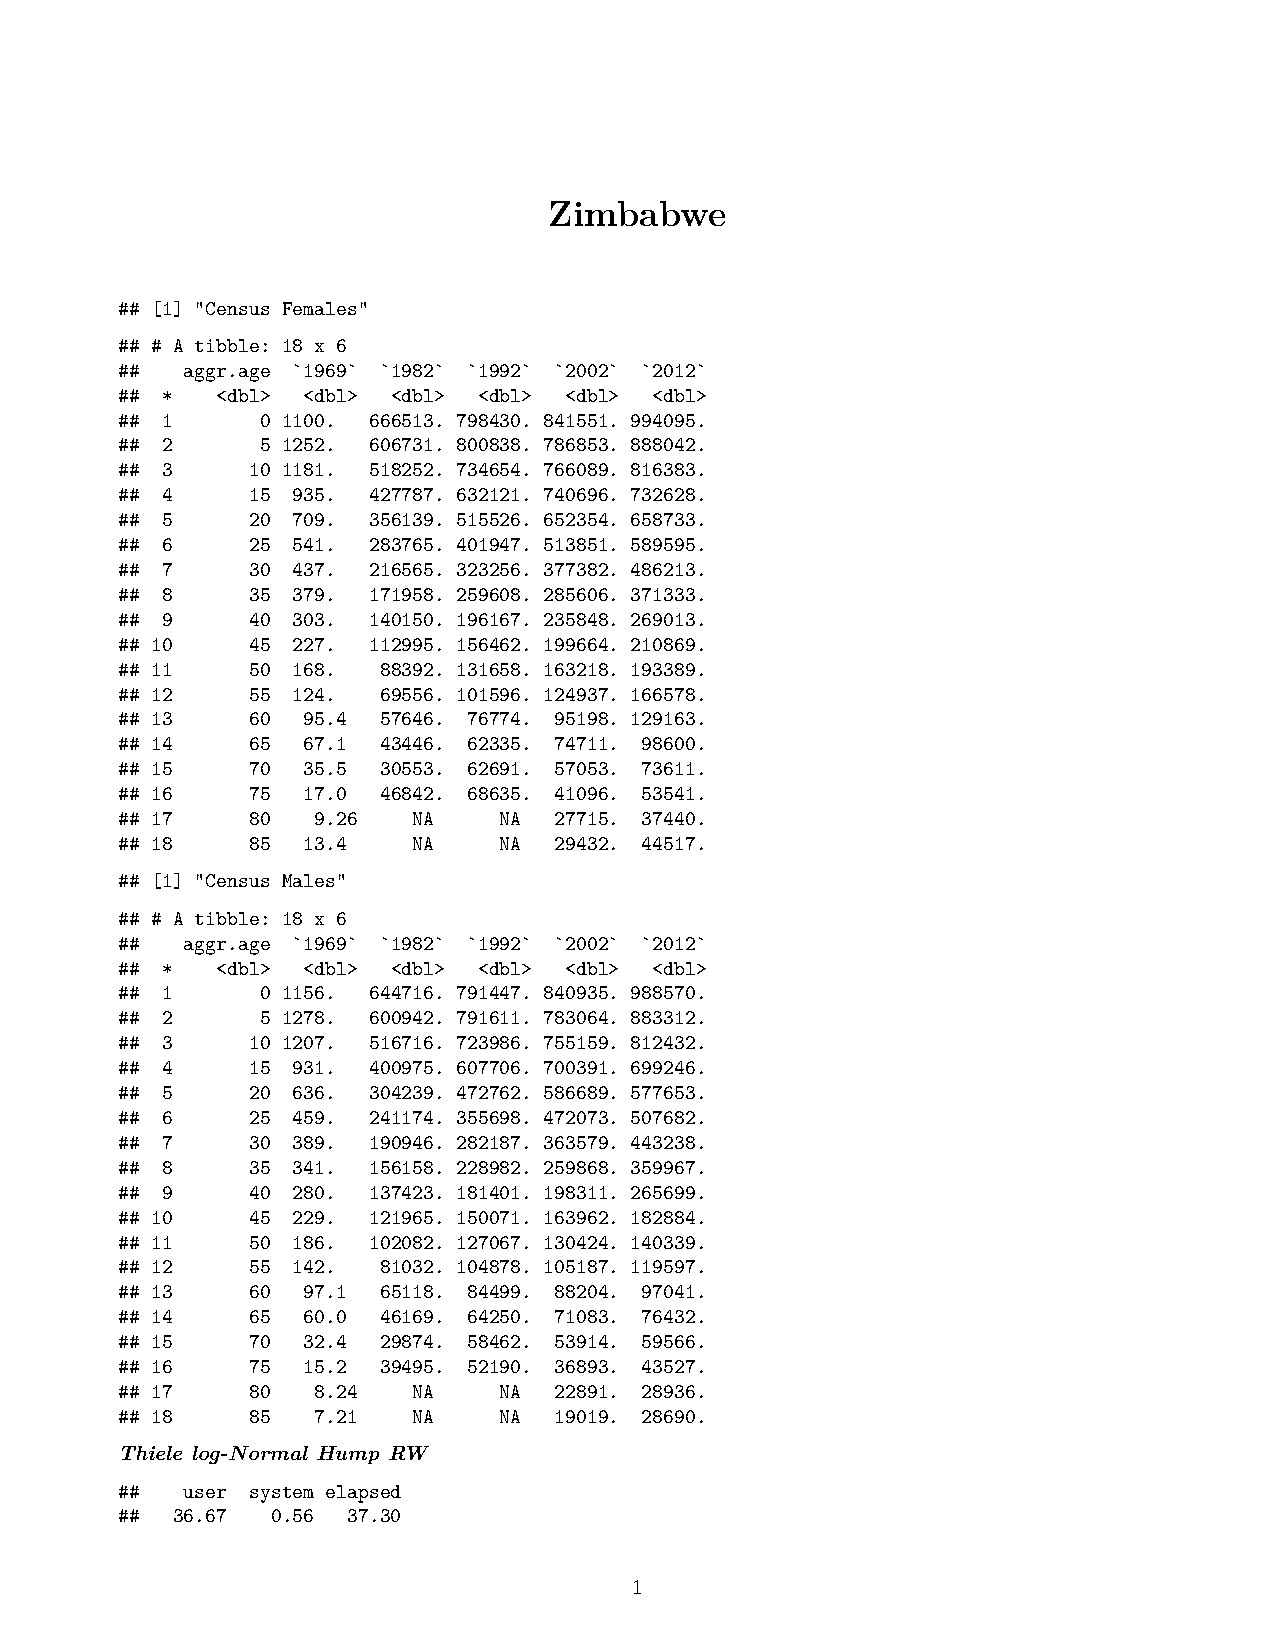
\includepdf[pages=-]{"../thiele_RW_Gumbel_1_and_5_common_AR2_phi_hiv_var_all/Zimbabwe.pdf"}

\end{document}